\documentclass[11pt,letterpaper]{article}
% draft is an option for the documentclass but it buys us nothing here. It only inhibits the importing of images.
\usepackage{minted}
\usepackage{booktabs}
\usepackage{graphicx}
\usepackage{hyperref,lineno}
\usepackage{datetime2}
\usepackage{amsmath,amssymb,amsfonts}
% Tweak the margin width to suit by changing the width of the text area.
%\usepackage[letterpaper, total={7in, 9in}]{geometry}
\usepackage[letterpaper, total={6.75in, 9in}]{geometry}
\usepackage[utf8]{inputenc}
\usepackage{setspace} \doublespacing
\usepackage[T1]{fontenc}
\usepackage{authblk}
\usepackage[labelfont=bf]{caption}
\DeclareCaptionType{equ}[][]

% cite package, to clean up citations in the main text. Do not remove.
\usepackage{cite}
%page numbers upper right
\pagestyle{myheadings}

\newenvironment{code}{\captionsetup{type=listing}}{}


% Approximate Arial font. To return to sans serif, uncomment the next two lines.
\usepackage{helvet}
\renewcommand{\familydefault}{\sfdefault}


\modulolinenumbers[1]
\bibliographystyle{cell}

% Remove brackets from numbering in List of References
\makeatletter
\renewcommand{\@biblabel}[1]{\quad#1.}
\makeatother

\title{Generic Manuscript Template}
\author[1]{Graduate Student}
\author[2]{Senior Collaborator}
\author[3]{Staff Scientist}
\author[1,2,3]{Blaine Mooers\thanks{blaine-mooers at ouhsc.edu, phone: 405-271-8XXX, FAX: 405-271-3X3X}}
\affil[1]{Department of Biochemistry and Molecular Biology, University of Oklahoma Health Sciences Center, Oklahoma City, Oklahoma, United States 73104}
\affil[2]{Stephenson Cancer Center, University of Oklahoma Health Sciences Center, Oklahoma City, Oklahoma, United States 73104}
\affil[2]{Laboratory of Biomolecular Structure and Function, University of Oklahoma Health Sciences Center, Oklahoma City, Oklahoma, United States 73104}



%%%%%%%%%%%%%%%%%%%%%%% End of the Preamable %%%%%%%%%%%%%%%%%%%%%%%%

\begin{document}

\maketitle


\newpage

\linenumbers

\begin{singlespace}
\section*{Abstract}
I draft the abstract after defining the scope of the paper with the Introduction and outlining the key results in the Results section and maybe the Discussion section.
I usually rewrite the abstract after the first draft is finished.
The abstract is often single-spaced.
I enclosed the abstract in the \emph{singlespace} environment.
\end{singlespace}



\paragraph{Keywords:} I draft the keywords in the writing document and select the best up to the allowable limit.

% A pox on those who over-use abbreviations! Unfamiliar ones slow-down the reader. Limit them to well-known ones.  
\paragraph{Abbreviations:} GUI: graphical user interface, IDE: integrated development environment 

\section*{Introduction}

% The Introduction is not a literature review.
% That is a separate class manuscript.

The first paragraph defines the scope of the problem and why it is important.
It might cite several key contributions in the area \cite{Newman2010TheC6WebToolAResourceForTheRationalSelectionOfCrystallizationConditions, Luft2007EfficientOptimizationOfCrystallizationConditionsByManipulationOfDropVolumeRatioAndTemperature}.
I like to use the author-year format to make it easier for the reviewers, irregardless of the required format.
Numbered formats are harder to look-up.
The last sentence should set up the first sentence of the next paragraph by hinting at possible approaches to the question or problem at hand.

The second paragraph starts with the central hypothesis that addressed the question or problem alluded to in paragraph one.
This is followed by a summary of our approach.
A sentence or two may be expended on a summary of what we found.
The last sentence describes the audience of the paper.



\section*{Materials and Methods}

This section is a series of subsections that may or may not in chronological order.
This section is often placed after the Discussion.

\section*{Results}

ParagraphOne: Map of the Results section. 
This introductory paragraph is usually missing, but no editor has ever asked me to delete it.
This paragraph tells the reader in a little more detail than the Introduction what they can expect to see and the order in which the results will be presented.


\subsection*{Most important result}
Cover results in declining importance relative to how they address the hypothesis. 
If they have no relevance, save them from another paper.
Chronological order is usually a poor choice.
End each paragraph with a conclusion.

Refer to tables and figures via their labels.
For example, see hot figure (Fig. \ref{fig:labelA}).
The numbering of the figures is handled automatically, so you can reorganize them without having to renumber them.

\subsection*{Second most important result}

See hot numbers in (Table \ref{tab:first}).
The numbering of the tables is handled automatically so you can reorganize them without having to renumber them.


\subsection*{Third most important result}

In-line equations are placed between dollar signs:  $y = mx + b$.
Display equations can be placed between double dollar signs or inside an equation environment.
These environments are not floats.
You can define a float and place them inside the float to enable the use of captions as I did below.
The \emph{equ} environment is defined in the preamble.



\begin{equ}[htp]  
\begin{equation}   
i \hbar \frac{d}{d t}|\Psi(t)\rangle=\hat{H}|\Psi(t)\rangle  
\end{equation}  
\caption{Eq. \label{Eq:first}Schrodinger's time-dependent wave equation.}   
\end{equ}

\subsection*{Fourth most important result}

Code listings also have to be enclosed inside floats to have captions.
The caption can be place above or below the code listng.

These environments need to be enclosed in the singlespace environment to retain single-line spacing in the code block.

The minted package provides the syntax highlighting.
The \mintinline{bash}{-shell-escape} must be used on compiling.



\begin{singlespace}
% Line numbering on and aligned with left margin. 
\begin{code}{}
  \index{openCV!measureSizes}
  \label{lst:measureSize}
  
\begin{minted}[frame=lines,
               framerule=2pt,
               linenos=true,
               xleftmargin=\parindent,
               breaklines]{python}
# import the necessary packages
from scipy.spatial import distance as dist
from imutils import perspective
from imutils import contours
import numpy as np
import argparse
import imutils
import cv2
 
def midpoint(ptA, ptB):
    return ((ptA[0] + ptB[0]) * 0.5, (ptA[1] + ptB[1]) * 0.5)

\end{minted}
\caption{\label{lst:size}Contents of measureSizes.py.}
\end{code}
\end{singlespace}

\subsection*{Fifth most important result}

\subsection*{Sixth most important result}

There could be up to four more subsections in a meaty paper.

There are usually four graphics and two tables in a minimal publishable unit.
This is a weak guideline because of the trend to use multipanel figures.
I have seen figures with ten or more panels.
Is it one figure or ten?

Delete all results that do not have a bearing on the central hypothesis or are less important.

\section*{Discussion}
How our results relate to the results of others.
(Avoid Results and Discussion sections: They do not work well. This is research paper, not a seminar).

Paragraph One: Map of the Discussion section. 
This paragraph is usually missing, but no editor has ever asked me to delete it.

Paragraphs two and beyond must end with a conclusion.
The conclusion can be a call to do more research.

Lay out the topics in declining importance.

Delete the paragraph with no bearing on the central hypothesis.


\section*{Acknowledgments}

Acknowledgments of core facilities and grant support. 
Double-check the grant numbers.
It is easy to make typos in these.
These acknowledgments are critical for the continued support of grants.


\bibliography{global}

\newpage
\listoftables
Tables should be one per page. 

The manual assembly of Tables is a challenge for beginners. 
Pandas, R, and the Python package latextable \url{https://github.com/JAEarly/latextable} can write out LaTeX tables. 
Tables are easy to assemble in org-mode in Emacs and exported to LaTeX. 
Markdown tables can be exported to LaTeX with pandoc. 
There are on-line tools to aid the assembly of LaTeX tables: \url{https://www.tablesgenerator.com/}.

The first table below was made with vanilla LaTeX.
The second table was made with the booktabs package: The horizontal rules are of different weights in the latter table.

There is a \emph{longtable} package for supporting tables that span more than one page.
It is also possible to have tables oriented in the landscape orientation via the \emph{lscape} package.



\newpage

\begin{table}[htp]
  \centering
  \caption{\label{tab:first} My summary statistics in the default LaTeX table. Dummy data.}
\begin{tabular}{lllll}\hline
 Parameter & Group A & Group B & Group C &  Group D \\ \hline
 Length ($\mu$m) & 100 & 150 & 175 &  250\\
 Weight (ng)  &  10 &  50 & 40  &  50\\
 Density (g/m) & 0.01  & 0.03  &  0.09 &  0.77\\ \hline
\end{tabular}
\end{table}


\newpage


\begin{table}[htp]
  \centering
  \caption{\label{tab:first} My summary statistics made with the booktabs package. Dummy data.}
\begin{tabular}{lllll}\toprule % l c and r control the alignment f the text in the table fields
 Parameter & Group A & Group B & Group C &  Group D \\ \midrule
 Length ($\mu$m) & 100 & 150 & 175 &  250\\
 Weight (ng)  &  10 &  50 & 40  &  50\\
 Density (g/m) & 0.01  & 0.03  &  0.09 &  0.77\\ \bottomrule
\end{tabular}
\end{table}


\newpage
\listoffigures
One figure per page. 

\newpage

\begin{figure}[htp]
  \begin{center}
  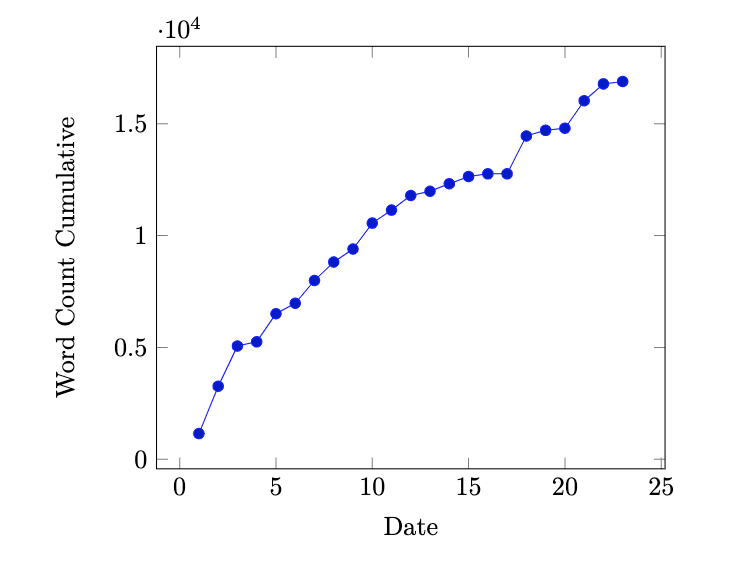
\includegraphics[width=3.25in]{./figs/wcPlot}
  \caption{\label{fig:labelA} This beautiful graph relates X to Y. }
  \end{center}
\end{figure}




\end{document}

%%% Local Variables:
%%% mode: latex
%%% TeX-master: t
%%% End:
